 \let\negmedspace\undefined
\let\negthickspace\undefined
\documentclass[journal]{IEEEtran}
\usepackage[a5paper, margin=10mm, onecolumn]{geometry}
\usepackage{lmodern} % Ensure lmodern is loaded for pdflatex
\usepackage{tfrupee} % Include tfrupee package

\setlength{\headheight}{1cm} % Set the height of the header box
\setlength{\headsep}{0mm}     % Set the distance between the header box and the top of the text

\usepackage{gvv-book}
\usepackage{gvv}
\usepackage{subfig}
\usepackage{cite}
\usepackage{amsmath,amssymb,amsfonts,amsthm}
\usepackage{algorithmic}
\usepackage{graphicx}
\usepackage{textcomp}
\usepackage{xcolor}
\usepackage{txfonts}
\usepackage{listings}
\usepackage{enumitem}
\usepackage{mathtools}
\usepackage{gensymb}
\usepackage{comment}
\usepackage[breaklinks=true]{hyperref}
\usepackage{tkz-euclide} 
\usepackage{listings}                                      
\def\inputGnumericTable{}                                 
\usepackage[latin1]{inputenc}                                
\usepackage{color}                                            
\usepackage{array}                                            
\usepackage{longtable}
\usepackage{multicol}
\usepackage{calc}                                             
\usepackage{multirow}                                         
\usepackage{hhline}                                           
\usepackage{ifthen}                                           
\usepackage{lscape}
\begin{document}

\bibliographystyle{IEEEtran}
\vspace{3cm}

\title{Digital Clock}
\author{EE24BTECH11052 - Rongali Charan}
% \maketitle
% \newpage
% \bigskip
{\let\newpage\relax\maketitle}

\renewcommand{\thefigure}{\theenumi}
\renewcommand{\thetable}{\theenumi}
\setlength{\intextsep}{10pt} % Space between text and floats


\numberwithin{equation}{enumi}
\numberwithin{figure}{enumi}
\renewcommand{\thetable}{\theenumi}
\tableofcontents
\newpage

\section{\textbf{Aim}}
Constructing the digital clock without using flipflops and using avr-gcc

    \section{ \textbf{Materials Required}}
\begin{itemize}
 \item 6x Common-anode 7-segment displays
    \item 7447 BCD-to-7-segment decoder
    \item 6x 180$\Omega$ resistors (for common anode current limiting)
    \item Jumper wires
    \item Bread Board
    \item Arduino UNO(atmega328p) and connecting cable
    \item Jumper wires for arduino and normal wires for seven segment displays
    \item Push Buttons
\end{itemize}
\section{Hardware Setup}
The wiring process involves connecting the 7447 decoder, segment lines, and common anodes to the Arduino pins.
\begin{figure}[H]
    \centering
    \subfloat[Seven Segment]{%
        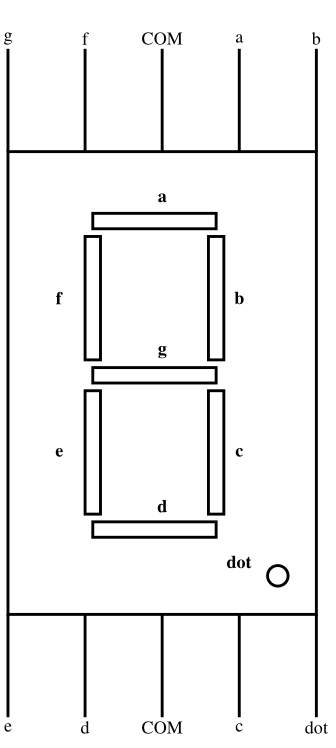
\includegraphics[width=0.3\textwidth]{Figs/Seven_seg.png}
        \label{fig:image1}
    }
    \hfill
    \subfloat[7447 Decoder]{%
        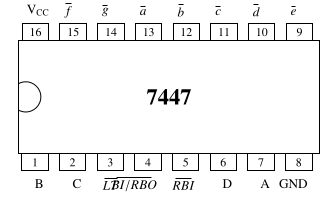
\includegraphics[width=0.45\textwidth]{Figs/decoder.png}
        \label{fig:image2}
    }
    \label{fig:main_figure}
\end{figure}



\subsection{7447 Connections}
The table below shows the connections between the 7447 decoder and the Arduino Uno:

\begin{table}[H]
    \centering
    \caption{7447 to Arduino Pin Connections}
    \begin{tabular}{|c|c|}
        \hline
        \textbf{7447 Pin} & \textbf{Arduino Connection} \\
        \hline
        VCC (Pin 16) & +5V \\
        GND (Pin 8) & GND \\
        A (Pin 7) & D2 (BCD input LSB) \\
        B (Pin 1) & D3 \\
        C (Pin 2) & D4 \\
        D (Pin 6) & D5 (BCD input MSB) \\
        \hline
    \end{tabular}
\end{table}

\subsection{Segment Connections}
The 7447 outputs are connected to the corresponding segments of all six displays, as shown in the table below:

\begin{table}[H]
    \centering
    \caption{7447 to Display Segment Connections}
    \begin{tabular}{|c|c|}
        \hline
        \textbf{7447 Pin} & \textbf{Display Segment} \\
        \hline
        Pin 13 & Segment "a" \\
        Pin 12 & Segment "b" \\
        Pin 14 & Segment "c" \\
        Pin 15 & Segment "d" \\
        Pin 9  & Segment "e" \\
        Pin 10 & Segment "f" \\
        Pin 11 & Segment "g" \\
        \hline
    \end{tabular}
\end{table}

\subsection{Common Anode Connections}
Each display's common anode is connected to an Arduino analog pin through a 180$\Omega$ resistor to limit current flow.

\begin{table}[H]
    \centering
    \caption{Common Anode Connections}
    \begin{tabular}{|c|c|}
        \hline
        \textbf{Display} & \textbf{Arduino Analog Pin (via 180$\Omega$ resistor)} \\
        \hline
        Display 1 & A0 \\
        Display 2 & A1 \\
        Display 3 & A2 \\
        Display 4 & A3 \\
        Display 5 & A4 \\
        Display 6 & A5 \\
        \hline
    \end{tabular}
\end{table}


\section{Key Design Notes}
\subsection{Current Limiting}
The 180$\Omega$ resistors on the common anodes limit the total current per digit. However, with all segments lit, each digit draws approximately:
\[
I = 7 \times 15\text{mA} = 105\text{mA}
\]
Since the Arduino analog pins are rated for 20mA max, prolonged operation could damage the board. Use brief testing sessions or add transistors to handle the higher current safely.

\subsection{Multiplexing}
The multiplexing ensures only one digit is active at a time. With a 2ms delay per digit, the full refresh cycle takes:
\[
6 \times 2\text{ms} = 12\text{ms}
\]
Brightness can be adjusted by modifying the delay value in the code.

\subsection{7447 Behavior}
The 7447 outputs are active-low, which means the segments turn on when the decoder outputs are LOW. This suits common-anode displays, which require low signals to activate the segments.

\section{Testing and Troubleshooting}

\subsection{Common Issues}
\begin{table}[H]
    \centering
    \caption{Troubleshooting Guide}
    \begin{tabular}{|c|c|}
        \hline
        \textbf{Problem} & \textbf{Solution} \\
        \hline
        Dim segments & Reduce resistor value (e.g., 100$\Omega$) \\
        Arduino overheating & Limit testing time or use transistors \\
        Incorrect digits & Verify BCD wiring order \\
        \hline
    \end{tabular}
\end{table}



\section{Code Implementation}
\section*{Key Features}
\begin{itemize}
    \item \textbf{Real-Time Interrupt-Driven Operation}: Timer1 is configured to trigger 1-second updates for consistent time management.
    \item \textbf{Interrupt Service Routine (ISR)}: Handles asynchronous updates to the Clock, Timer, and Stopwatch modes.
    \item \textbf{Multiplexed Display Control}: Efficient hardware management using binary-coded decimal (BCD) encoding and multiplexing.
    \item \textbf{Debounced Buttons}: Smooth user interaction for adjusting time settings and controlling modes.
    \item \textbf{Dynamic Mode Switching}: Seamlessly switches between Clock, Timer, and Stopwatch functionality using a mode variable.
\end{itemize}

\section*{ISR Overview}
The \textbf{Interrupt Service Routine (ISR)} is the backbone of the program, ensuring precise real-time operations. The Timer1 interrupt triggers every second, enabling reliable timekeeping and supporting the following functionalities:
\begin{itemize}
    \item \textbf{Clock Mode}: Implements a simple incrementing mechanism using \textbf{modulo arithmetic}, where seconds roll over after 60, minutes after 60, and hours after 24.
    \item \textbf{Timer Mode}: Uses a nested logic structure to decrement seconds, minutes, and hours. Special conditions ensure smooth transitions when seconds or minutes reach zero.
    \item \textbf{Stopwatch Mode}: Implements incrementing logic with rollover at 60 seconds and 60 minutes, similar to the Clock Mode. This is done to track elapsed time efficiently.
    \item \textbf{Debugging with PC7}: Toggles the \textbf{debugging LED} to ensure the ISR is running correctly and at expected intervals.
\end{itemize}

\section*{Hardware Overview}
\begin{itemize}
    \item \textbf{Registers}: \texttt{TCCR1B}, \texttt{OCR1A}, \texttt{PORTD}, \texttt{PORTC}, and \texttt{PINB}.
    \item \textbf{7-Segment Display}: Controlled using binary-coded decimal (BCD) encoding.
    \item \textbf{Buttons}: Connected to \texttt{PD6}, \texttt{PD7}, and \texttt{PB0/PB1} for mode switching and adjustments.
\end{itemize}

\section*{Code Snippets}
\subsection*{Timer Setup}
\begin{lstlisting}[language=C, frame=single, basicstyle=\ttfamily\small, keywordstyle=\color{blue}]
TCCR1B |= (1 << WGM12) | (1 << CS12) | (1 << CS10);
OCR1A = 15625; // 1-second interrupt
TIMSK1 |= (1 << OCIE1A);
sei(); // Enable global interrupts
\end{lstlisting}

\subsection*{Interrupt Service Routine (ISR)}
\begin{lstlisting}[language=C, frame=single, basicstyle=\ttfamily\small, keywordstyle=\color{blue}]
ISR(TIMER1_COMPA_vect) {
    // Toggle a debug LED to check ISR functionality
    PORTC ^= (1 << 7);

    // Clock Mode Logic
    if (mode == 0) { 
        seconds++;
        if (seconds == 60) { 
            seconds = 0; 
            minutes++; 
            if (minutes == 60) {
                minutes = 0;
                hours = (hours + 1) % 24; 
            }
        }
    }

    // Timer Countdown Logic
    if (mode == 1 && stopwatch_running) {
        if (timer_seconds > 0 || timer_minutes > 0 || timer_hours > 0) {
            if (timer_seconds == 0) {
                if (timer_minutes > 0) {
                    timer_minutes--;
                    timer_seconds = 59;
                } else if (timer_hours > 0) {
                    timer_hours--;
                    timer_minutes = 59;
                    timer_seconds = 59;
                }
            } else {
                timer_seconds--;
            }
        }
    }

    // Stopwatch Increment Logic
    if (mode == 2 && stopwatch_running) {
        stopwatch_seconds++;
        if (stopwatch_seconds == 60) {
            stopwatch_seconds = 0;
            stopwatch_minutes++;
            if (stopwatch_minutes == 60) {
                stopwatch_minutes = 0;
                stopwatch_hours = (stopwatch_hours + 1) % 24;
            }
        }
    }
}
\end{lstlisting}



\subsection*{Multiplexed Display Control}
\begin{lstlisting}[language=C, frame=single, basicstyle=\ttfamily\small, keywordstyle=\color{blue}]
void displayTime() {
    int digits[6];

    if (mode == 0) { // Clock Mode
        digits[0] = hours / 10;
        digits[1] = hours % 10;
        digits[2] = minutes / 10;
        digits[3] = minutes % 10;
        digits[4] = seconds / 10;
        digits[5] = seconds % 10;
    } else if (mode == 1) { // Timer Mode
        // Timer digits logic
    } else { // Stopwatch Mode
        // Stopwatch digits logic
    }

    // Multiplex 7-segment display
    for (int i = 0; i < 6; i++) {
        setBCD(digits[i]); // Send the BCD value
        COMMON_PORT = (1 << i); // Enable the corresponding digit
        _delay_us(500); // Short delay for smooth display
    }
}
\end{lstlisting}
\section{Special Logic Implemented}
\begin{itemize}
    \item \textbf{State Management Using Conditional Logic}:
    \begin{itemize}
    \item The `mode` variable acts as a state machine, with values 0, 1, and 2 corresponding to Clock, Timer, and Stopwatch modes, respectively.
    \item Logical separation of functionality is achieved using `if-else` conditions within the ISR.
    \end{itemize}

    \item \textbf{Efficient Timing with Timer1 Interrupts}:
    \begin{itemize}
    \item Timer1 is configured in CTC Mode, where the timer triggers the ISR every second. This eliminates reliance on delay functions or main loop polling.
    \end{itemize}

    \item \textbf{Modular Countdown and Increment Logic}:
    \begin{itemize}
    \item  The Timer Mode implements a cascading decrement mechanism: seconds decrement until zero, at which point minutes or hours are adjusted.
     \item This cascading logic mimics the behavior of a **ripple counter** often seen in digital hardware design.
     \end{itemize}

    \item \textbf{Persistence of Vision (Multiplexing)}:\\Uses a sequential activation of each digit on the 7-segment display, controlled through a multiplexing mechanism with BCD encoding. This reduces the number of required microcontroller pins.
\end{itemize}
\section{Conclusion}
This setup allows efficient control of six 7-segment displays using a single Arduino Uno and a 7447 decoder. However, be mindful of the current limits and use transistors for safer, prolonged operation.\\
The main logic of this program demonstrates an efficient, interrupt-driven design for a timekeeping system. By leveraging state management and modular timekeeping logic, the system provides robust functionality with minimal resource usage. Key aspects like cascading decrement logic for the timer and multiplexed display control highlight the elegance of combining hardware and software in embedded systems.
\begin{figure}[h!]
    \centering
    \subfloat[Clock]{%
        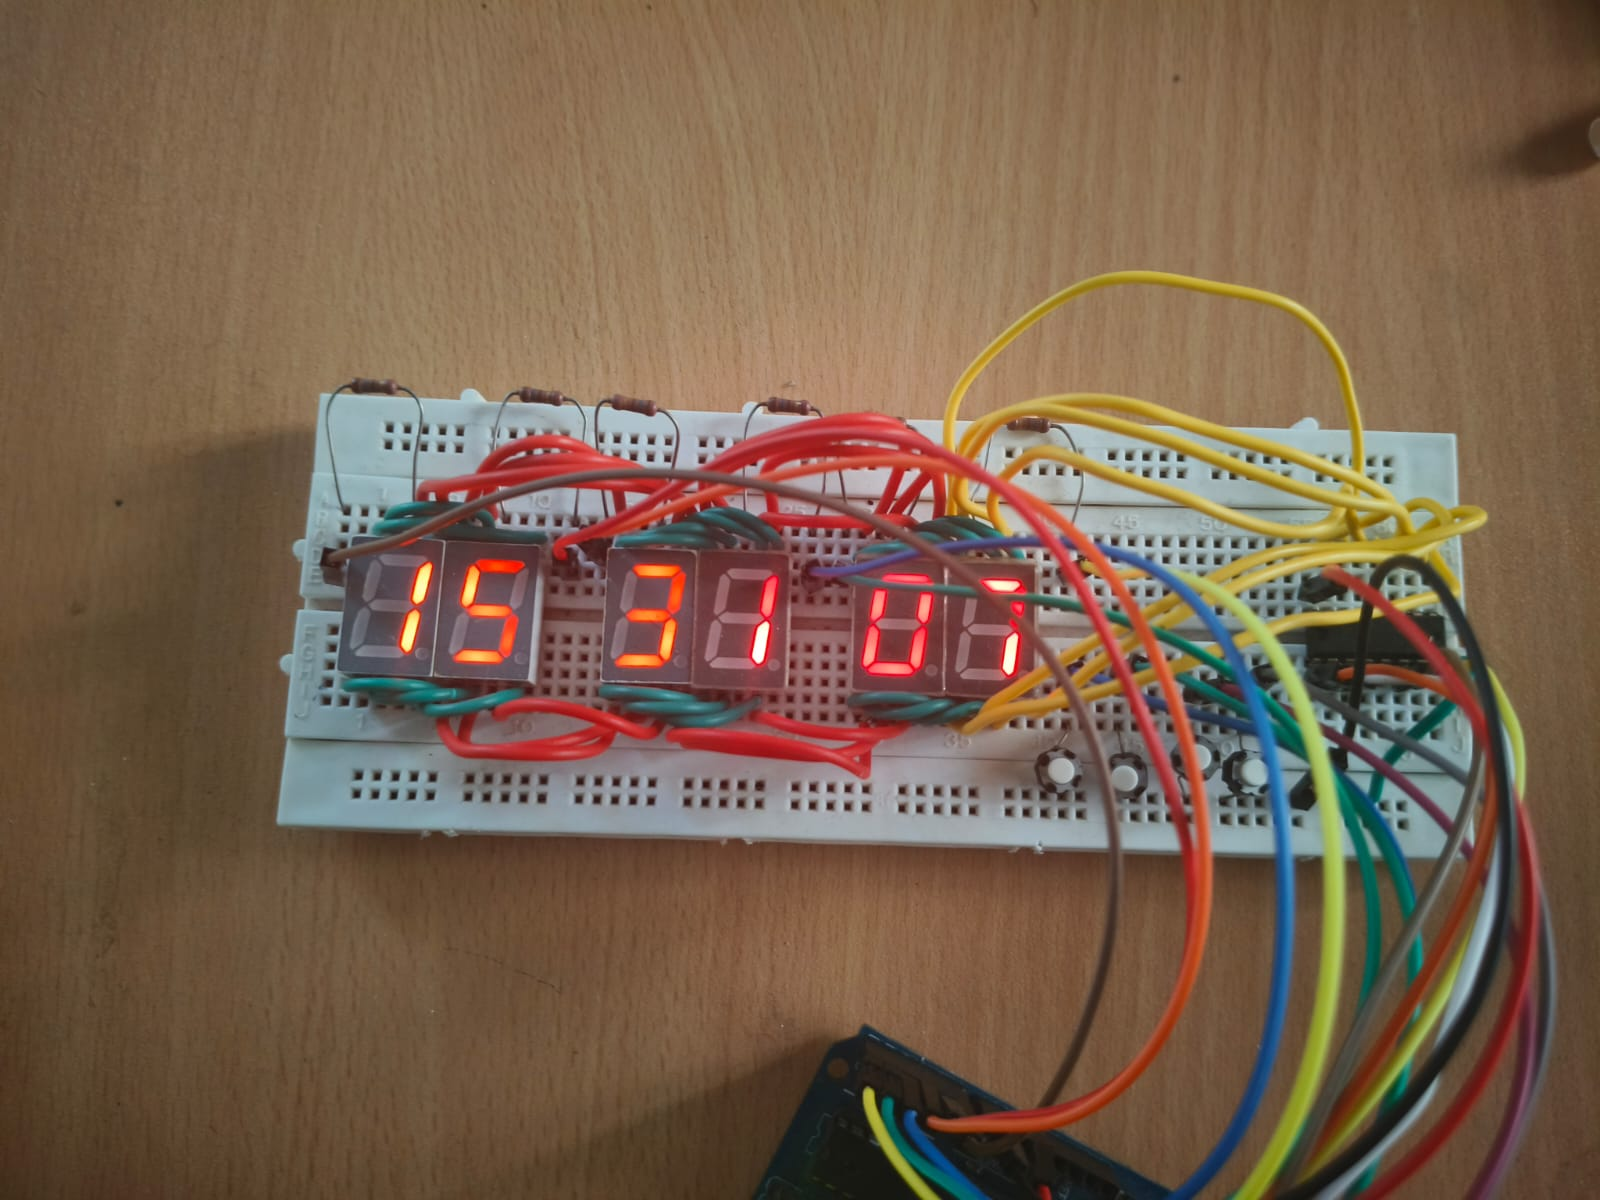
\includegraphics[width=0.32\textwidth]{Figs/Clock.png}
        \label{fig:fig1}
    }
    \hfill
    \subfloat[Timer]{%
        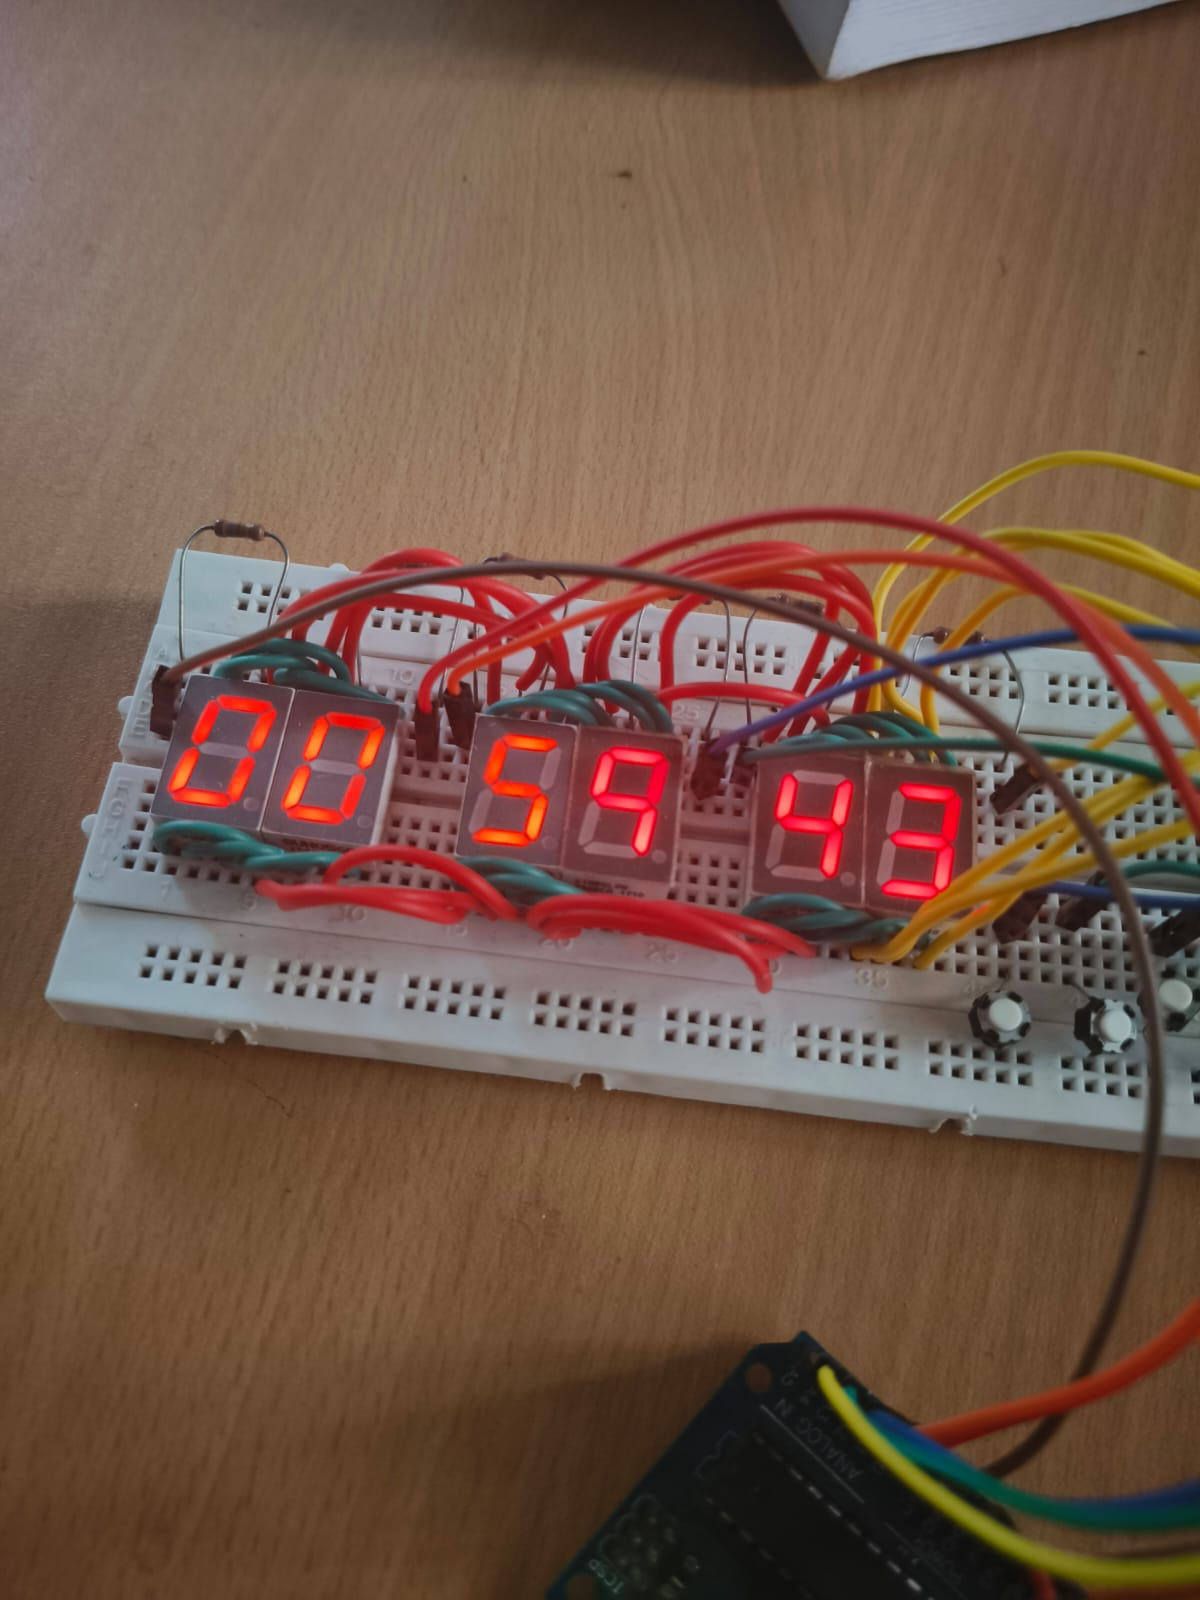
\includegraphics[width=0.32\textwidth]{Figs/Timer.png}
        \label{fig:fig2}
    }
    \hfill
    \subfloat[Stopwatch]{%
        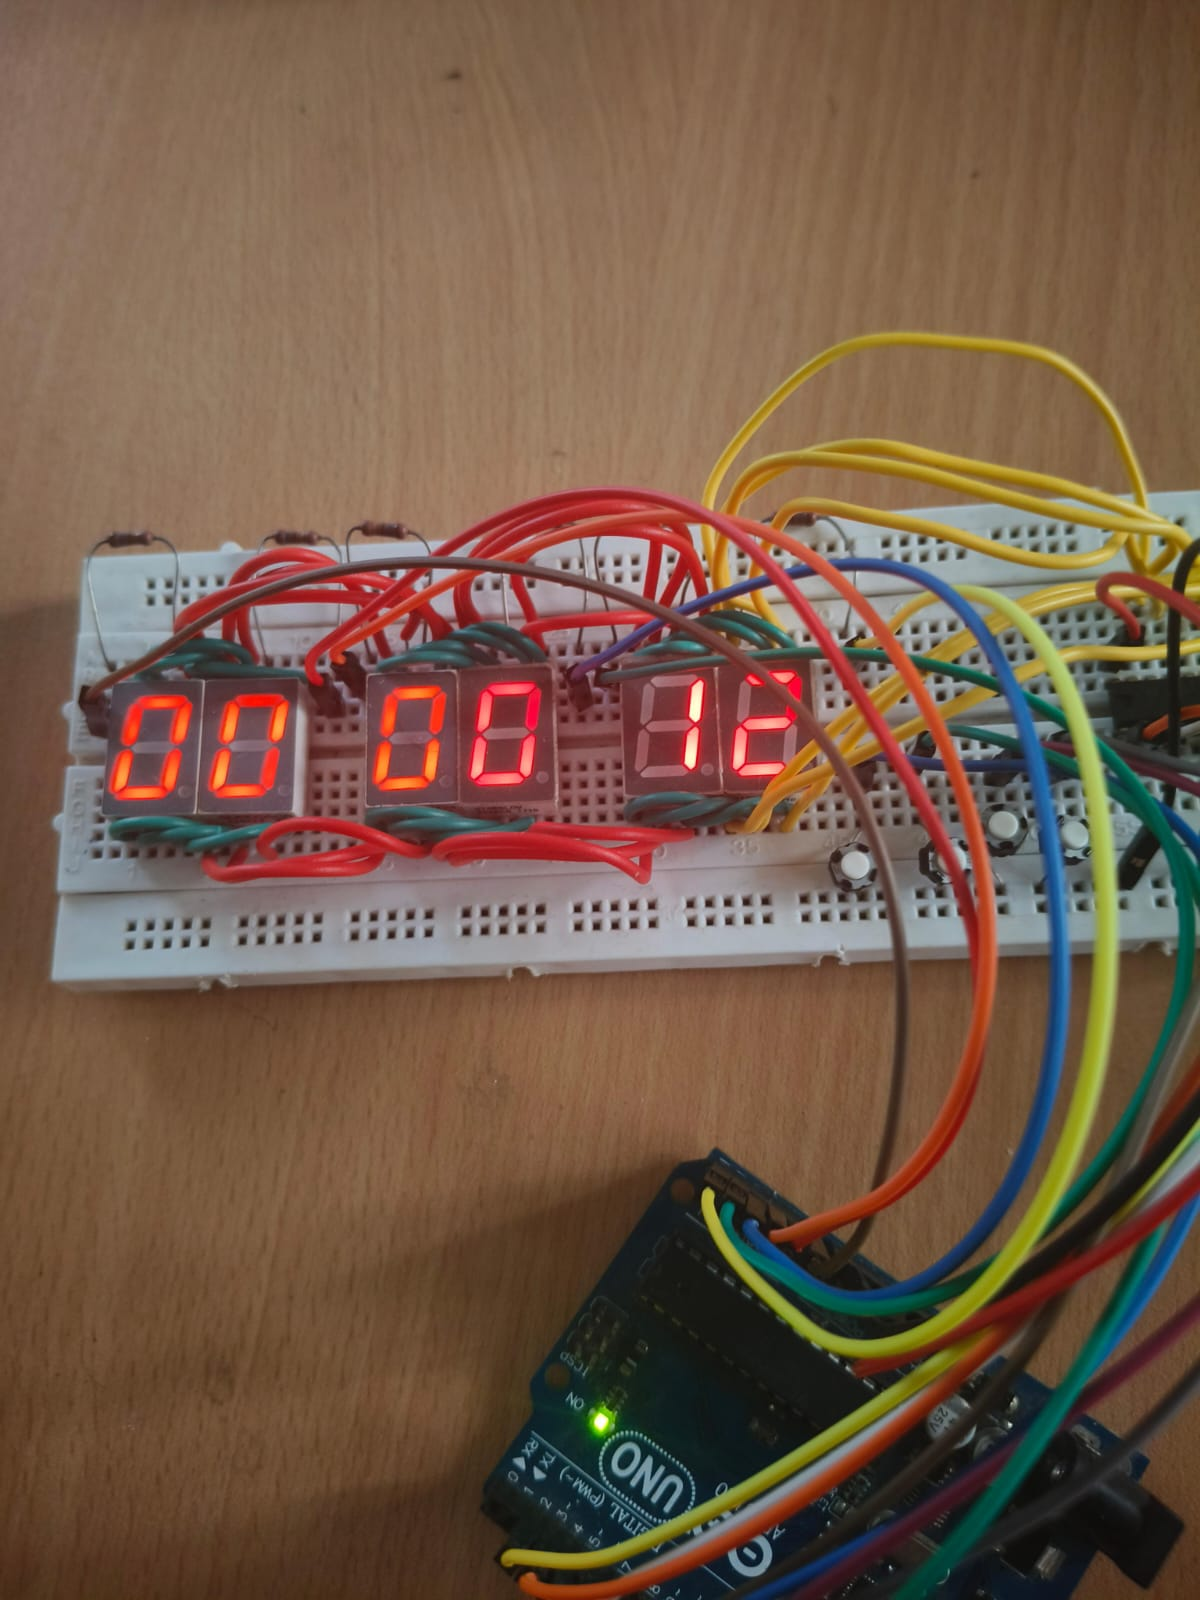
\includegraphics[width=0.32\textwidth]{Figs/Stopwatch.png}
        \label{fig:fig3}
    }
    \label{fig:main_fig}
\end{figure}


\end{document}


%\end{document}
